\documentclass[11pt, a4paper]{article}\usepackage[]{graphicx}\usepackage[]{color}
%% maxwidth is the original width if it is less than linewidth
%% otherwise use linewidth (to make sure the graphics do not exceed the margin)
\makeatletter
\def\maxwidth{ %
  \ifdim\Gin@nat@width>\linewidth
    \linewidth
  \else
    \Gin@nat@width
  \fi
}
\makeatother

\definecolor{fgcolor}{rgb}{0.345, 0.345, 0.345}
\newcommand{\hlnum}[1]{\textcolor[rgb]{0.686,0.059,0.569}{#1}}%
\newcommand{\hlstr}[1]{\textcolor[rgb]{0.192,0.494,0.8}{#1}}%
\newcommand{\hlcom}[1]{\textcolor[rgb]{0.678,0.584,0.686}{\textit{#1}}}%
\newcommand{\hlopt}[1]{\textcolor[rgb]{0,0,0}{#1}}%
\newcommand{\hlstd}[1]{\textcolor[rgb]{0.345,0.345,0.345}{#1}}%
\newcommand{\hlkwa}[1]{\textcolor[rgb]{0.161,0.373,0.58}{\textbf{#1}}}%
\newcommand{\hlkwb}[1]{\textcolor[rgb]{0.69,0.353,0.396}{#1}}%
\newcommand{\hlkwc}[1]{\textcolor[rgb]{0.333,0.667,0.333}{#1}}%
\newcommand{\hlkwd}[1]{\textcolor[rgb]{0.737,0.353,0.396}{\textbf{#1}}}%

\usepackage{framed}
\makeatletter
\newenvironment{kframe}{%
 \def\at@end@of@kframe{}%
 \ifinner\ifhmode%
  \def\at@end@of@kframe{\end{minipage}}%
  \begin{minipage}{\columnwidth}%
 \fi\fi%
 \def\FrameCommand##1{\hskip\@totalleftmargin \hskip-\fboxsep
 \colorbox{shadecolor}{##1}\hskip-\fboxsep
     % There is no \\@totalrightmargin, so:
     \hskip-\linewidth \hskip-\@totalleftmargin \hskip\columnwidth}%
 \MakeFramed {\advance\hsize-\width
   \@totalleftmargin\z@ \linewidth\hsize
   \@setminipage}}%
 {\par\unskip\endMakeFramed%
 \at@end@of@kframe}
\makeatother

\definecolor{shadecolor}{rgb}{.97, .97, .97}
\definecolor{messagecolor}{rgb}{0, 0, 0}
\definecolor{warningcolor}{rgb}{1, 0, 1}
\definecolor{errorcolor}{rgb}{1, 0, 0}
\newenvironment{knitrout}{}{} % an empty environment to be redefined in TeX

\usepackage{alltt} %or article has only section and below, book and report also have chapter: http://texblog.org/2007/07/09/documentclassbook-report-article-or-letter/

\usepackage[utf8]{inputenc}  % use utf8 encoding of symbols such as umlaute for maximal compatibility across platforms

\usepackage{caption}				% provides commands for handling caption sizes etc.
%\usepackage[a4paper, left=25mm, right=20mm, top=25mm, bottom=20mm]{geometry}		 % to easily change margin widths: https://www.sharelatex.com/learn/Page_size_and_margins

\usepackage{etoolbox}    % for conditional evaluations!
\usepackage[bottom]{footmisc}  % I love footnotes! And they should be down at the bottom of the page!
\usepackage{graphicx}        % when using figures and alike
\usepackage[hidelinks]{hyperref}		% for hyperreferences (links within the document: references, figures, tables, citations)

\usepackage{euler}     % a math font, only for equations and alike; call BEFORE changing the main font; alternatives: mathptmx, fourier, 
%\usepackage{gentium} % for a different font; you can also try: cantarell, charter, libertine, gentium, bera, ... http://tex.stackexchange.com/questions/59403/what-font-packages-are-installed-in-tex-live

%------------------------------------------------------------------------------------------------------
%------- text size settings --------------
\setlength{\textwidth}{16cm}% 
\setlength{\textheight}{25cm} %23 
%(these values were used to fill the page more fully and thus reduce the number of pages!)
\setlength{\topmargin}{-1.5cm} %0
\setlength{\footskip}{1cm} %
%\setlength{\hoffset}{0cm} %
\setlength{\oddsidemargin}{1cm}%
\setlength{\evensidemargin}{-.5cm}%
\setlength{\parskip}{0cm} % Abstand zwischen Absätzen
% ----------------------------------------------------------------
\renewcommand{\textfraction}{0.1} % allows more space to graphics in float
\renewcommand{\topfraction}{0.85}
%\renewcommand{\bottomfraction}{0.65}
\renewcommand{\floatpagefraction}{0.70}


\frenchspacing %http://texwelt.de/wissen/fragen/1154/was-ist-french-spacing-was-macht-frenchspacing
%------------------------------------------------------------------------------------------------------
%------------------------------------------------------------------------------------------------------
\IfFileExists{upquote.sty}{\usepackage{upquote}}{}
\begin{document}
%\SweaveOpts{concordance=TRUE}
%%%%%%%%%%%%% this bit is new to Knitr: %%%%%%%%%%%%%%%%%%%%%



\title{A tutorial for Step Selection Function}

\author{P. Antkowiak\thanks{M.Sc. programme "GIS und Umweltmodellierung" at University of Freiburg} \and H. Tripke\thanks{M.Sc. programme "Wildlife, Biodiversity and Vegetation" at University of Freiburg} \and C. Wilhelm\thanks{M.Sc. programme "Wildlife, Biodiversity and Vegetation" at University of Freiburg}}
% for more control, multiple affiliations, line breaks and alike, use the authblk package!!

\date{\today} % !!use package isodate for more control of date formatting!!

\maketitle

%------------------------------------------------------------------------------------------------------
%------------------------------------------------------------------------------------------------------

\tableofcontents

\newpage

\section{Introduction}%------------------------------------------------------------------------------------------------------
In addition to Resources Selection Functions (RSF) a more detailed anlysis for telemetry data can be conducted by using Step Selection Function (SSF). The use of latter is providing answers to th actual selection of animals on their habitat rather than analysing the use of a habitat only. (DO WE WANT TO CITE, HERE FOR EXAMPLE Simone and friends). So far most of the SSF were done in GIS to use spatial data together with mathematics equations. However, more and more packages are provided in R and thus becomes a valuable alternative. \
This tutorial provides an overview on how to implement SSF with R. The main package we will use in the following is the package \textbf{adehabitatLT}. All single steps that need to be taken care of are summarized in (Figure~\ref{fig:Flowchart}).


\begin{figure} % you can (but shouldn't) use [h] behind {figure} to force the picture to go here. However, the idea of LaTeX is that it will do things for you, so too much interfering is not saving you any time.
% see also here: http://en.wikibooks.org/wiki/LaTeX/Floats,_Figures_and_Captions#Captions
\captionsetup{width=1\textwidth}
\centering
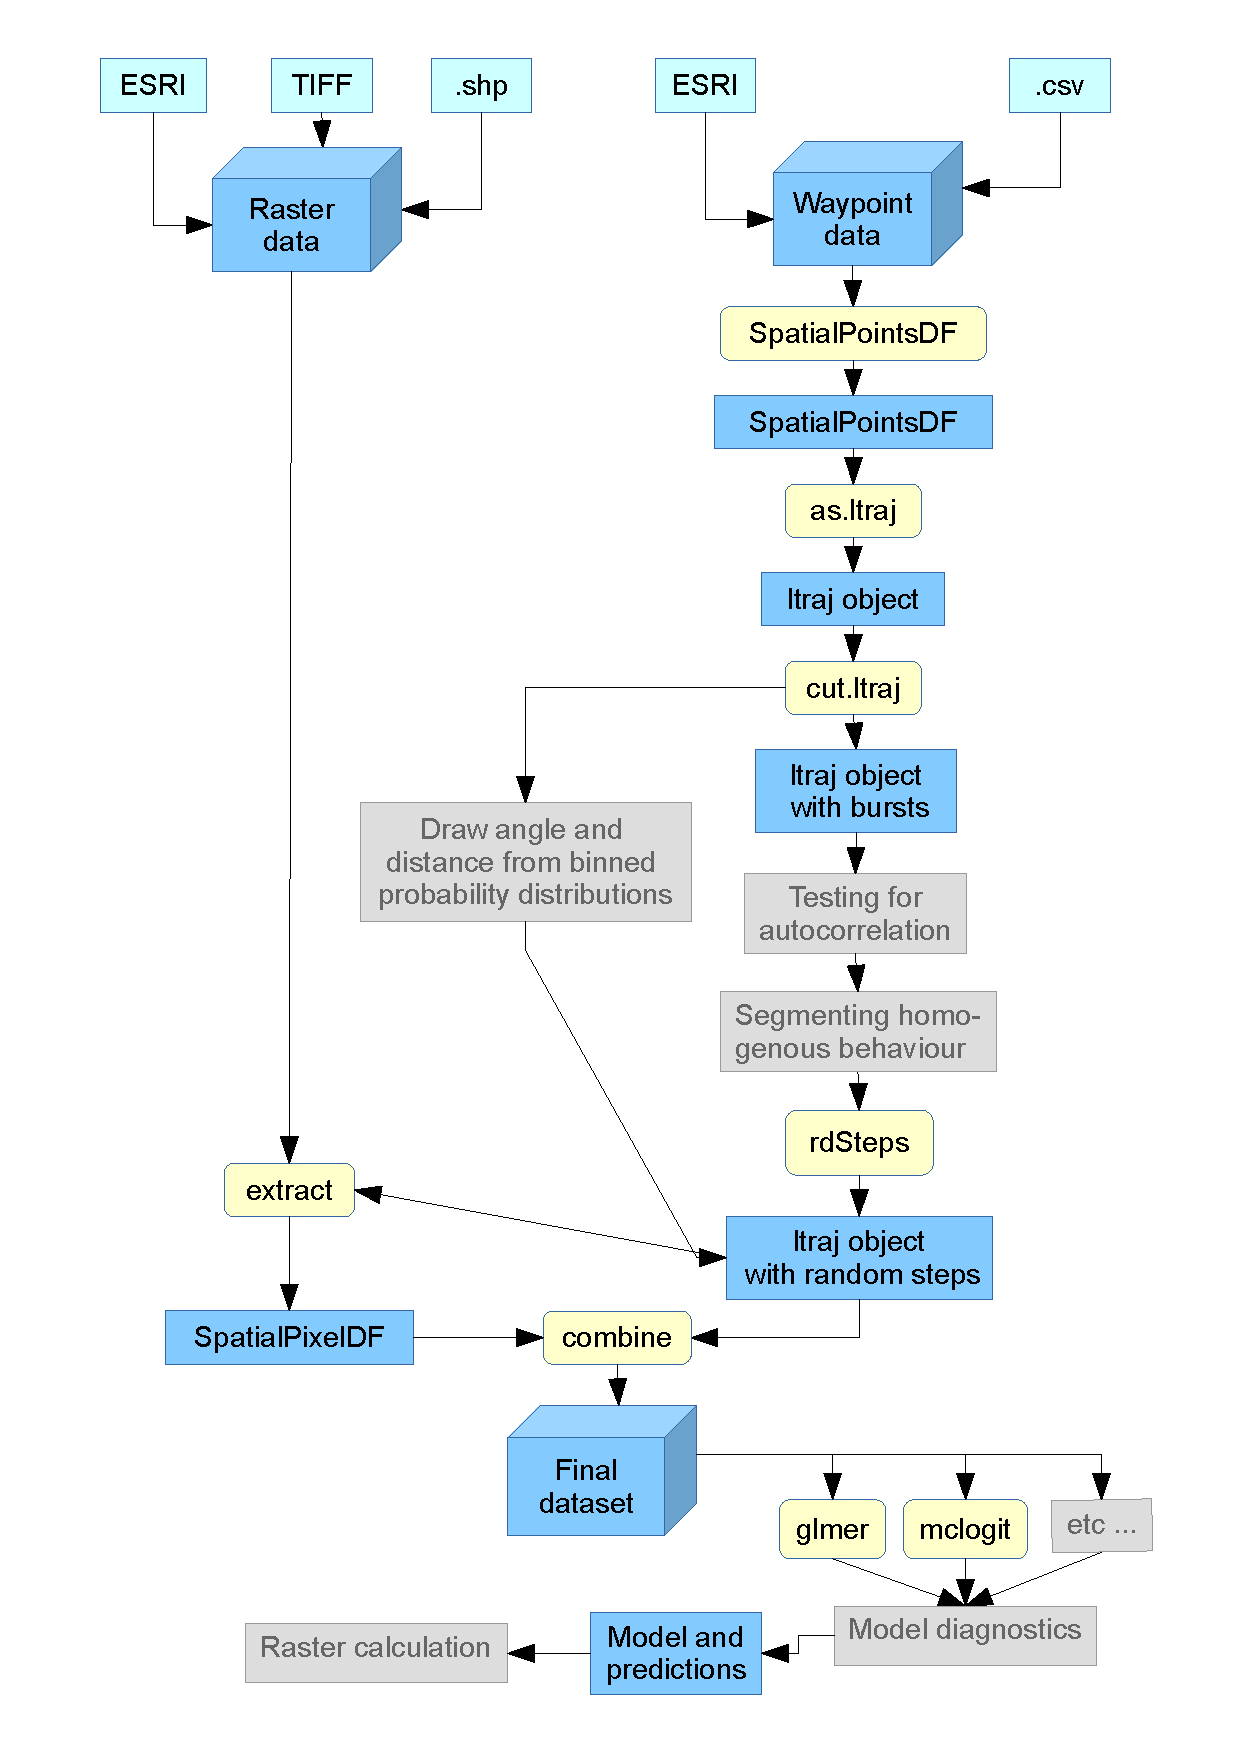
\includegraphics[width=1\textwidth]{Flowchart.pdf} %our perfect workflow!
\caption{\emph{Conducting a SSF using existing R-packages:} this figures provides an overview of the steps necessary to conduct a SSF. The steps are separated in subsections, which the turtorial will guide you through.}
\label{fig:Flowchart}
\end{figure}




\section{Preparations}
Before you can actually start using the tutorial for conducting SSF you need to load a bunch of packages in R. Some of them require others so that you have to add all these to your library:

\subsection{Packages - what we need}

\begin{knitrout}
\definecolor{shadecolor}{rgb}{0.969, 0.969, 0.969}\color{fgcolor}\begin{kframe}
\begin{alltt}
\hlcom{# installing packages -----------------------------------------------------}

\hlcom{# install.packages("adehabitat")}

\hlcom{# install.packages("hab")}
\hlkwd{install.packages}\hlstd{(}\hlstr{"hab"}\hlstd{,} \hlkwc{repos} \hlstd{=} \hlstr{"http://ase-research.org/R/"}\hlstd{,} \hlkwc{type} \hlstd{=} \hlstr{"source"}\hlstd{)}
\hlcom{# install.packages("hab", repos = "http://ase-research.org/R/")}

\hlkwd{install.packages}\hlstd{(}\hlstr{"adehabitatMA"}\hlstd{)}
\hlkwd{install.packages}\hlstd{(}\hlstr{"adehabitatHR"}\hlstd{)}
\hlkwd{install.packages}\hlstd{(}\hlstr{"adehabitatHS"}\hlstd{)}
\hlkwd{install.packages}\hlstd{(}\hlstr{"adehabitatLT"}\hlstd{)} \hlcom{# will be installed when insatlling adehabitatHR}
\hlkwd{install.packages}\hlstd{(}\hlstr{"tkrplot"}\hlstd{)}


\hlkwd{require}\hlstd{(hab)}
\hlkwd{require}\hlstd{(adehabitatMA)}
\hlkwd{require}\hlstd{(adehabitatLT)}  \hlcom{# includes "ade4"}
\hlkwd{require}\hlstd{(adehabitatHS)}
\hlkwd{require}\hlstd{(tkrplot)}

\hlcom{# require(adehabitat)  # not necessary to load}
\end{alltt}
\end{kframe}
\end{knitrout}


\section{Load raster data (ESRI, *.tif, *.shp)}%------------------------------------------------------------------------------------------------------


\section{Extract coordinates for comparison of used and random points} %------------------------------------------------------------------------------------------------------
Peter is successfully doing this step!!

\section{Load telemetry data (*.csv, ESRI)}%------------------------------------------------------------------------------------------------------
The data for the analysis is should be safed in a simple *.csv format. Depending on your analysis you have to include 
\begin{enumerate}
\item{coordinates}
\item{ID}
\item{date and/or time}
\end{enumerate}

\section{Create a Spatial Points Data Frame}%------------------------------------------------------------------------------------------------------

\section{Create a ltraj object}%------------------------------------------------------------------------------------------------------
 

\section{Compute random steps}


\section{Final SSF model}


Don't forget to thank TeX and R and other opensource communities if you use their products! The correct way to cite R is shown when typing ``\texttt{citation()}'', and ``\texttt{citation("mgcv")}'' for packages.






\newpage
\section{still useful code from Carsten}

 I left this in there cause we might need the help when adding our code...

\begin{verbatim}
# This is how I could document code:
runif(100)
# but it only contains the code and can also run over the line, as shown here ...
# convenient for short, but not for long pieces of code
# any symbol is plotted "as is", even if it is \LaTeX: *+#&ß\/
\end{verbatim}

# any symbol is plotted "as is", even if it is \LaTeX: *+#&ß\/


Alternatively, in Sweave, I can actually use R-code and have it evaluated by R and results returned and pasted into the \LaTeX-document! Like so:
\begin{knitrout}
\definecolor{shadecolor}{rgb}{0.969, 0.969, 0.969}\color{fgcolor}\begin{kframe}
\begin{alltt}
\hlkwd{runif}\hlstd{(}\hlnum{10}\hlstd{)}
\end{alltt}
\begin{verbatim}
##  [1] 0.9829789 0.5495859 0.5235186 0.2654087 0.1903815 0.6912136 0.8983265 0.2532187
##  [9] 0.5575985 0.7742271
\end{verbatim}
\end{kframe}
\end{knitrout}
Or I can only have the code returned, but \textbf{not} evaluated (useful if it takes a long time, or if results are produced externally beforehand):
\begin{knitrout}
\definecolor{shadecolor}{rgb}{0.969, 0.969, 0.969}\color{fgcolor}\begin{kframe}
\begin{alltt}
\hlkwd{runif}\hlstd{(}\hlnum{10}\hlstd{)}
\end{alltt}
\end{kframe}
\end{knitrout}
Similarly, I can have the code evaluated but the call not returned:
\begin{knitrout}
\definecolor{shadecolor}{rgb}{0.969, 0.969, 0.969}\color{fgcolor}\begin{kframe}
\begin{verbatim}
##  [1] 0.56906532 0.37986997 0.73346162 0.06215843 0.64431340 0.90812612 0.45775895
##  [8] 0.51576533 0.43007653 0.14327208
\end{verbatim}
\end{kframe}
\end{knitrout}
To combine both, simply add both options, separated by a ``,''.

You can also put an R-expression into the text. For example, the mean of 10 random number between 0 and 1 is (in this simulation) 0.63, rounded to 3 digits. This value will change every time you compile this document.

Finally, you can first do the computations, store them (in R objects) and then refer to them in the text.

\begin{knitrout}
\definecolor{shadecolor}{rgb}{0.969, 0.969, 0.969}\color{fgcolor}\begin{kframe}
\begin{verbatim}
## 
## 	Pearson's product-moment correlation
## 
## data:  X and Y
## t = 1.9196, df = 8, p-value = 0.09117
## alternative hypothesis: true correlation is not equal to 0
## 95 percent confidence interval:
##  -0.1052939  0.8800316
## sample estimates:
##       cor 
## 0.5615616
\end{verbatim}
\end{kframe}
\end{knitrout}
So, the correlation between X and Y is    not significant, and the mean of Y is 1.

\bigskip

\noindent So that's all cool, and the only thing we also could wish for is to produce figures and insert them into the text automatically:

\begin{knitrout}
\definecolor{shadecolor}{rgb}{0.969, 0.969, 0.969}\color{fgcolor}\begin{kframe}
\begin{alltt}
\hlkwd{hist}\hlstd{(}\hlkwd{rnorm}\hlstd{(}\hlnum{100}\hlstd{),} \hlkwc{col}\hlstd{=}\hlstr{"grey"}\hlstd{,} \hlkwc{border}\hlstd{=}\hlstr{"white"}\hlstd{,} \hlkwc{las}\hlstd{=}\hlnum{1}\hlstd{)}
\end{alltt}
\end{kframe}

{\centering 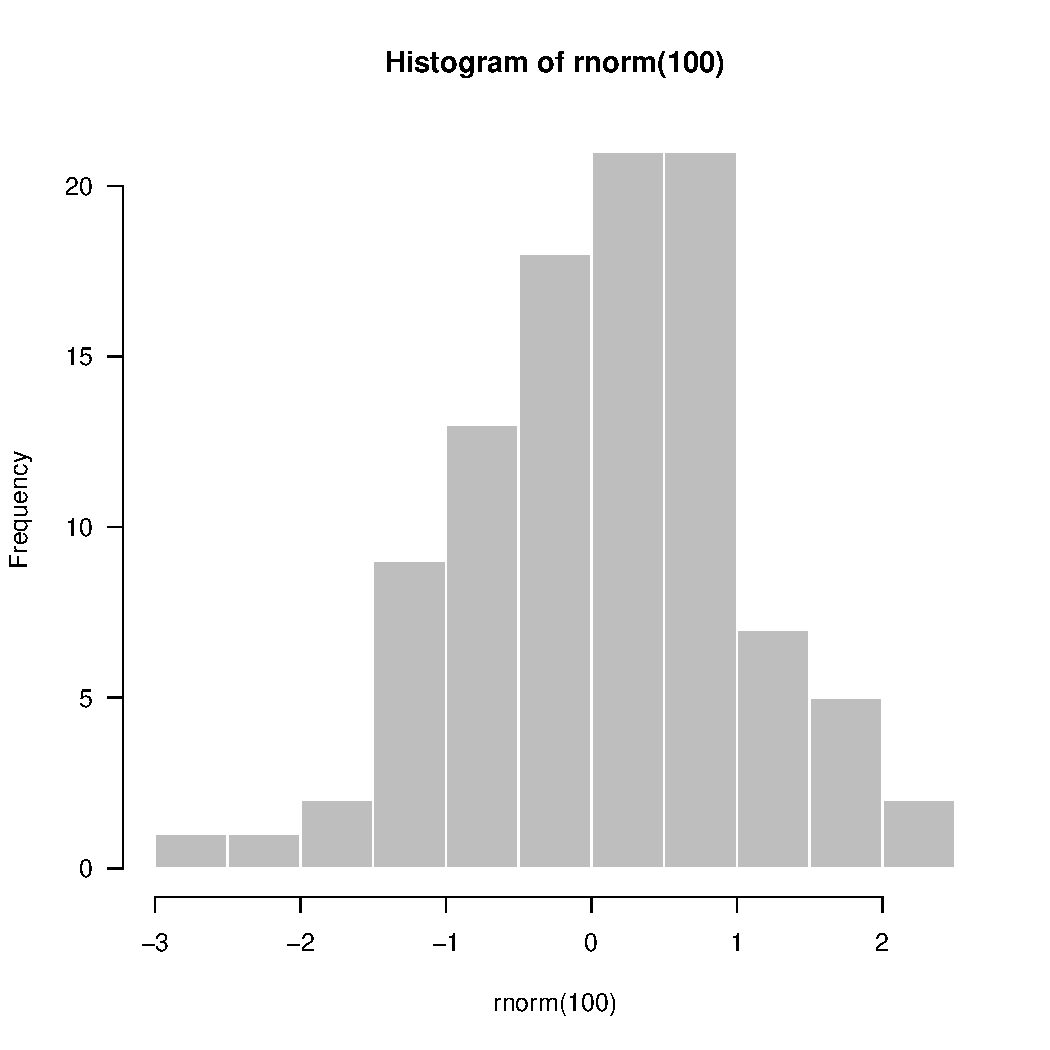
\includegraphics[width=\maxwidth]{unnamed-chunk-6-1} 

}



\end{knitrout}

We may want to ``hide'' the figure generating text and show the result in a float-environment with a proper caption. To do so, we only have to wrap the above code in a figure environment, like so:
\begin{verbatim}
\begin{figure}
\centering
#<<label=fig2plot, echo=FALSE, fig=TRUE>>=
hist(rnorm(100), col="grey", border="white", las=1)
#@
\caption{This is an example figure, computed and immediately returned.}
\end{figure}
\end{verbatim}
Notice that I only put the \texttt{\#} in to prevent R from evaluating the code. In a real document, you would NOT do that.

Now one minor issue is that you cannot readily change the size of this figure. The best way to do this is to split the figure-generating process up into two part: one generates the figure and saves it as PDF, then we use standard \LaTeX\/to load this figure. Like so:\footnote{Obviously in the document you would have to remove the \#s.}
\begin{verbatim}
#<<anexamplehistogram, echo=FALSE, dev="pdf">>=
hist(rnorm(100), col="cornflowerblue", border="white", las=1)
#@

\begin{figure}
\centering
\includegraphics[width=0.5\textwidth]{anexamplehistogram}
\caption{This is an example figure, exported as PDF and then, on loading, 
  scaled to half the text's width.}
\end{figure}
\end{verbatim}

\begin{figure}
\centering
\includegraphics[width=0.5\textwidth]{anexamplehistogram}
\captionsetup{width=0.8\textwidth}
\caption{This is an example figure, exported as PDF and then, on loading, scaled to half the text's width.}
\end{figure}


\medskip

I leave it to you to do the same thing for tables, using R's xtable command, as illustrated in the Sweave demo of Friedrich Leisch (\url{users.stat.umn.edu/~geyer/Sweave/foo.pdf}).


All this was Sweave. More recently, knitr made its entrance, and has increased the flexibility of Sweave. It is VERY similar and you have to tell RStudio in the options, whether you are sweaving or knitting. For minimal examples and comparisons, also using markdown rather than \LaTeX\/and PDF or html as output, see here: \url{http://yihui.name/knitr/demo/minimal/}.

\end{document}
